\documentclass[11pt,letterpaper]{article}
\usepackage[utf8]{inputenc}
\usepackage[T1]{fontenc}
\usepackage[spanish]{babel}
\usepackage{amsmath,amssymb}
\usepackage{graphicx}
\usepackage{booktabs}
\usepackage{float}
\usepackage[margin=2.2cm]{geometry}
\usepackage{hyperref}

\title{\textbf{Integración de Teoría de la Información y Sistemas de Comunicación en un Sistema de Telemetría y Monitoreo Remoto de Frecuencia Cardíaca}}
\author{Alejandro Rodríguez Arciniegas \and Daniel Oñate Hernández}
\date{Noviembre de 2026}

\begin{document}
\maketitle

\begin{abstract}
Se presenta el diseño, modelado matemático y simulación integral de la cadena de procesamiento y transmisión digital de información aplicada a un sistema embebido de telemetría cardíaca basado en microcontroladores ESP32-S3 Mini y ESP32. El desarrollo abarca desde el acondicionamiento espectral de la señal fotopletismográfica (PPG) y su conversión analógica-digital mediante Modulación por Codificación de Pulsos (PCM), hasta la transmisión en banda base, compresión sin pérdida mediante codificación de Huffman sobre los estados operativos del paciente y protección contra ruido AWGN mediante códigos lineales de bloque Hamming $(7,4)$.
\end{abstract}

\section{Arquitectura Sistémica del Enlace de Telemetría (Capítulo I)}
El sistema opera bajo una arquitectura desacoplada entre la capa de hardware embebido (Nodo Sensor con ESP32-S3 Mini, servidor MQTT/API y Nodo Monitor con ESP32, pantalla, botonera y servomotor) y la cadena de comunicaciones digitales simulada en MATLAB:
\begin{equation*}
\text{Fuente PPG/Estados} \rightarrow \text{Filtro Pasa-Banda} \rightarrow \text{Muestreo y PCM} \rightarrow \text{Cod. Huffman} \rightarrow \text{Hamming }(7,4) \rightarrow \text{Canal AWGN}
\end{equation*}
Cada trama discreta generada por el nodo sensor empaqueta $17\text{ bits}$: $2\text{ bits}$ para el estado operativo (\texttt{NORMAL}, \texttt{SIN\_DETECCION}, \texttt{ALERTA\_BAJA}, \texttt{ALERTA\_ALTA}), $8\text{ bits}$ para la lectura de frecuencia cardíaca (BPM) y $7\text{ bits}$ para el nivel de batería LiPo.

\section{Análisis Espectral y Filtrado Digital de Señales PPG (Capítulo II)}
La señal fisiológica capturada a $F_{s,\text{sim}} = 1000\text{ Hz}$ presenta componente fundamental cardíaca $f_0 = \text{BPM}/60 \approx 1.25\text{ Hz}$, armónicos dicróticos, deriva de línea base por movimiento ($0.2\text{ Hz}$) y ruido aditivo. Mediante la Transformada Rápida de Fourier (FFT) unilateral se determinó el ancho de banda efectivo $W = 3.80\text{ Hz}$ que concentra el $99\%$ de la potencia útil en la banda cardíaca, aplicando un filtro Butterworth pasa-banda de fase cero ($0.5\text{ Hz}$ a $W$).

\begin{figure}[H]
    \centering
    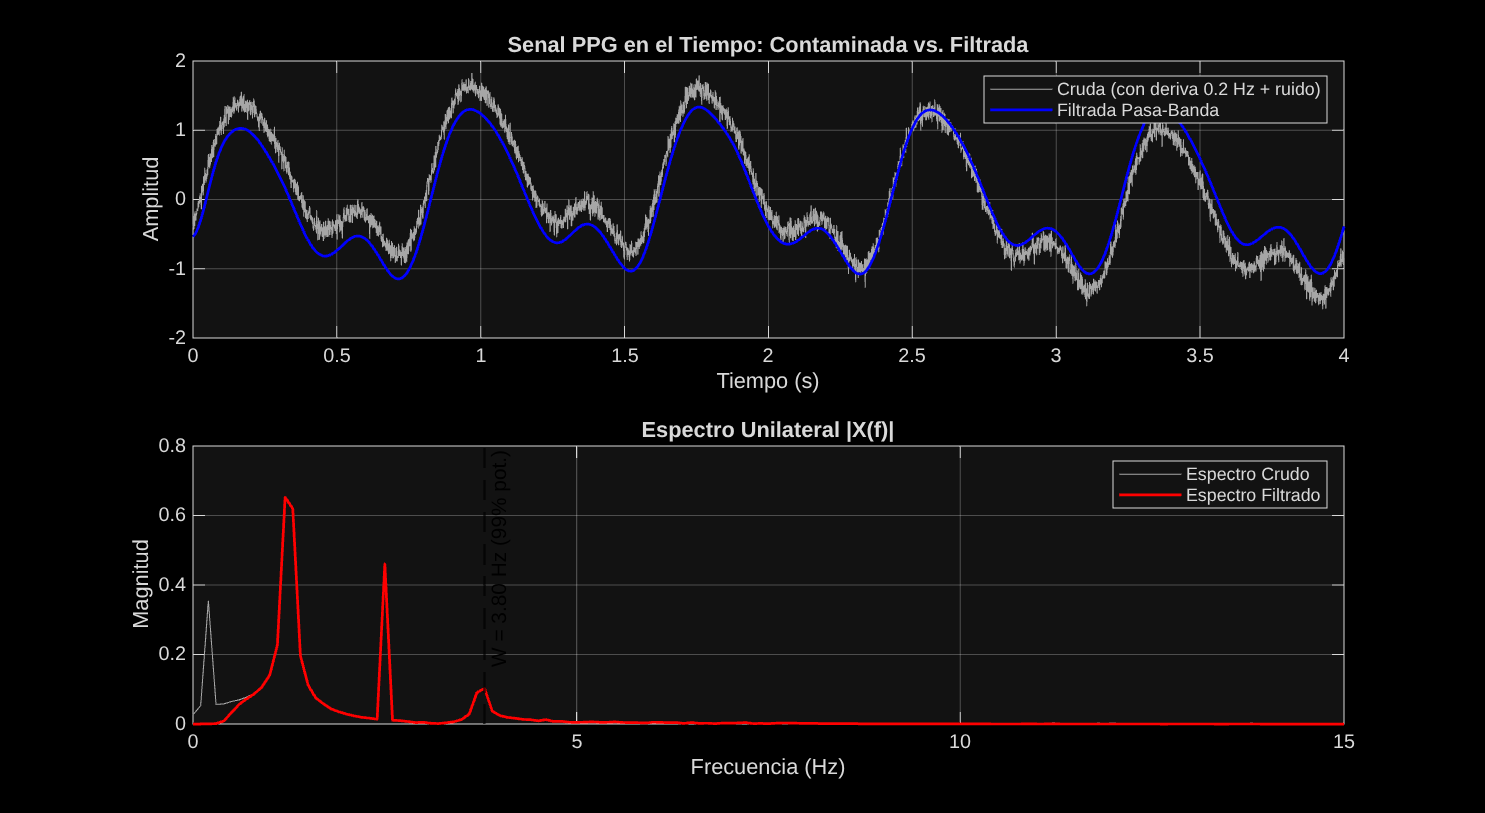
\includegraphics[width=0.92\textwidth]{figs/paso2_espectral.png}
    \caption{Señal PPG en dominio del tiempo (izquierda/arriba) y espectro unilateral $|X(f)|$ antes y después del filtrado pasa-banda (abajo).}
    \label{fig:espectral}
\end{figure}

\section{Muestreo de Nyquist, Cuantización PCM y Banda Base (Capítulo III)}
\subsection{Teorema de Nyquist y Relación Señal a Ruido de Cuantización (SQNR)}
Para evitar solapamiento espectral (\textit{aliasing}), la frecuencia de muestreo del ADC debe satisfacer $F_s \ge 2W = 7.60\text{ Hz}$. Se validó el muestreo adecuado a $F_s = 50\text{ Hz}$ frente al submuestreo con \textit{aliasing} a $F_s = 4\text{ Hz}$. Asimismo, para una cuantización uniforme de $b$ bits con paso $\Delta = (x_{\max}-x_{\min})/2^b$, se contrastó la $\text{SQNR}$ experimental frente a la cota teórica:
\begin{equation}
\text{SQNR}_{\text{dB}} = 10\log_{10}\left(\frac{P_{\text{señal}}}{P_{\text{error}}}\right) \approx 6.02\,b + 1.76\text{ [dB]}
\end{equation}

\begin{figure}[H]
    \centering
    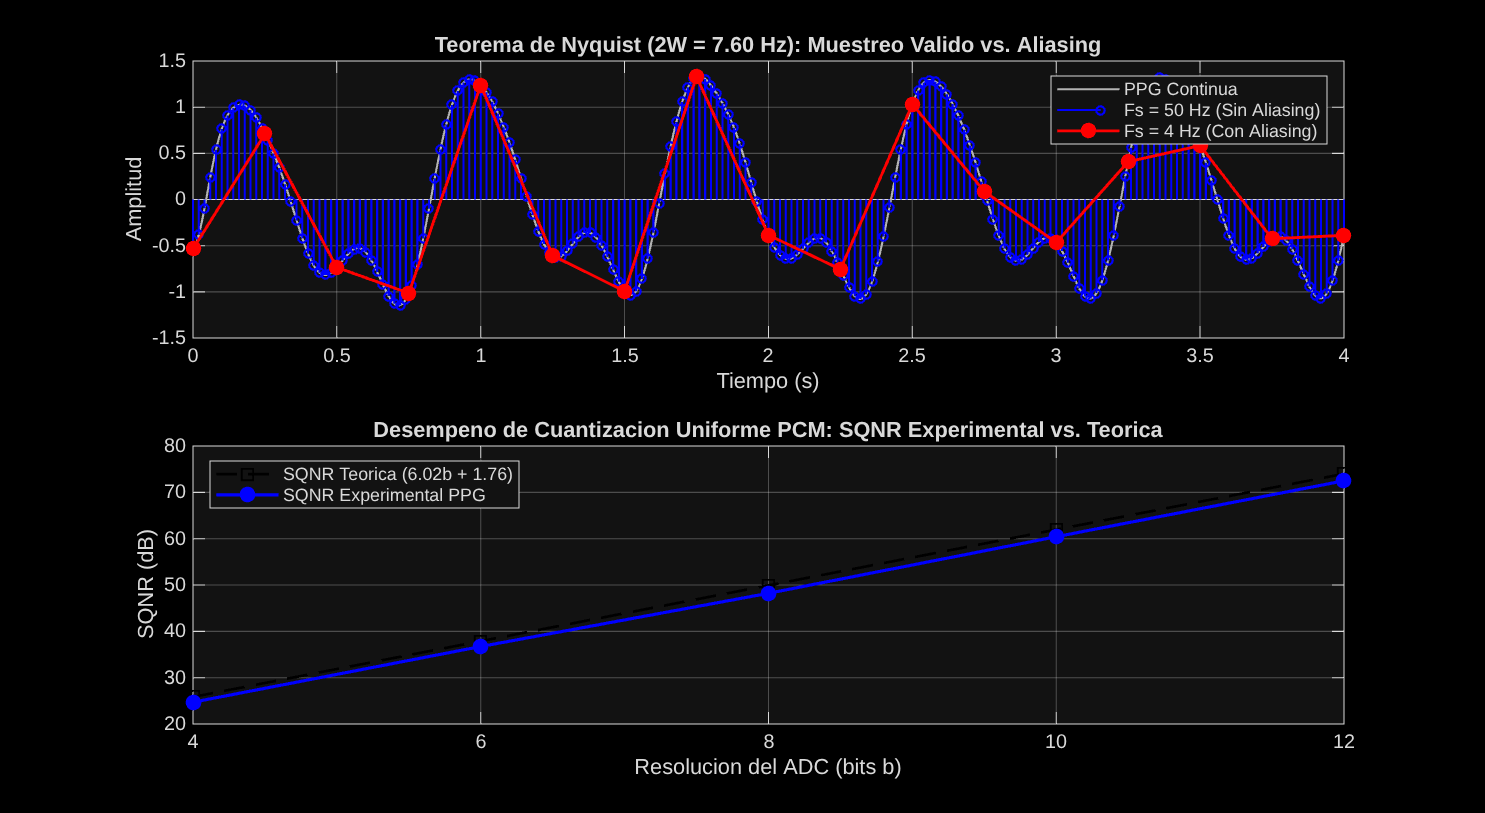
\includegraphics[width=0.92\textwidth]{figs/paso3_pcm.png}
    \caption{Verificación del criterio de Nyquist ($F_s = 50\text{ Hz}$ vs. $4\text{ Hz}$) y curva de desempeño $\text{SQNR}$ para $b \in \{4,6,8,10,12\}\text{ bits}$.}
    \label{fig:pcm}
\end{figure}

\subsection{Codificación de Línea, Densidad Espectral de Potencia e ISI}
Se compararon los esquemas NRZ Polar y Manchester a $R_b = 1\text{ kbps}$. Manchester elimina la componente DC en $f = 0\text{ Hz}$ y garantiza transiciones de sincronización a mitad de bit a costa de duplicar el ancho de banda nulo ($2R_b$ frente a $R_b$). Al transmitir NRZ por un canal pasa-bajas limitado en banda ($f_c = 0.75\,R_b$) con ruido AWGN, el diagrama de ojo evidencia la apertura vertical (margen de ruido) en los instantes óptimos de muestreo.

\begin{figure}[H]
    \centering
    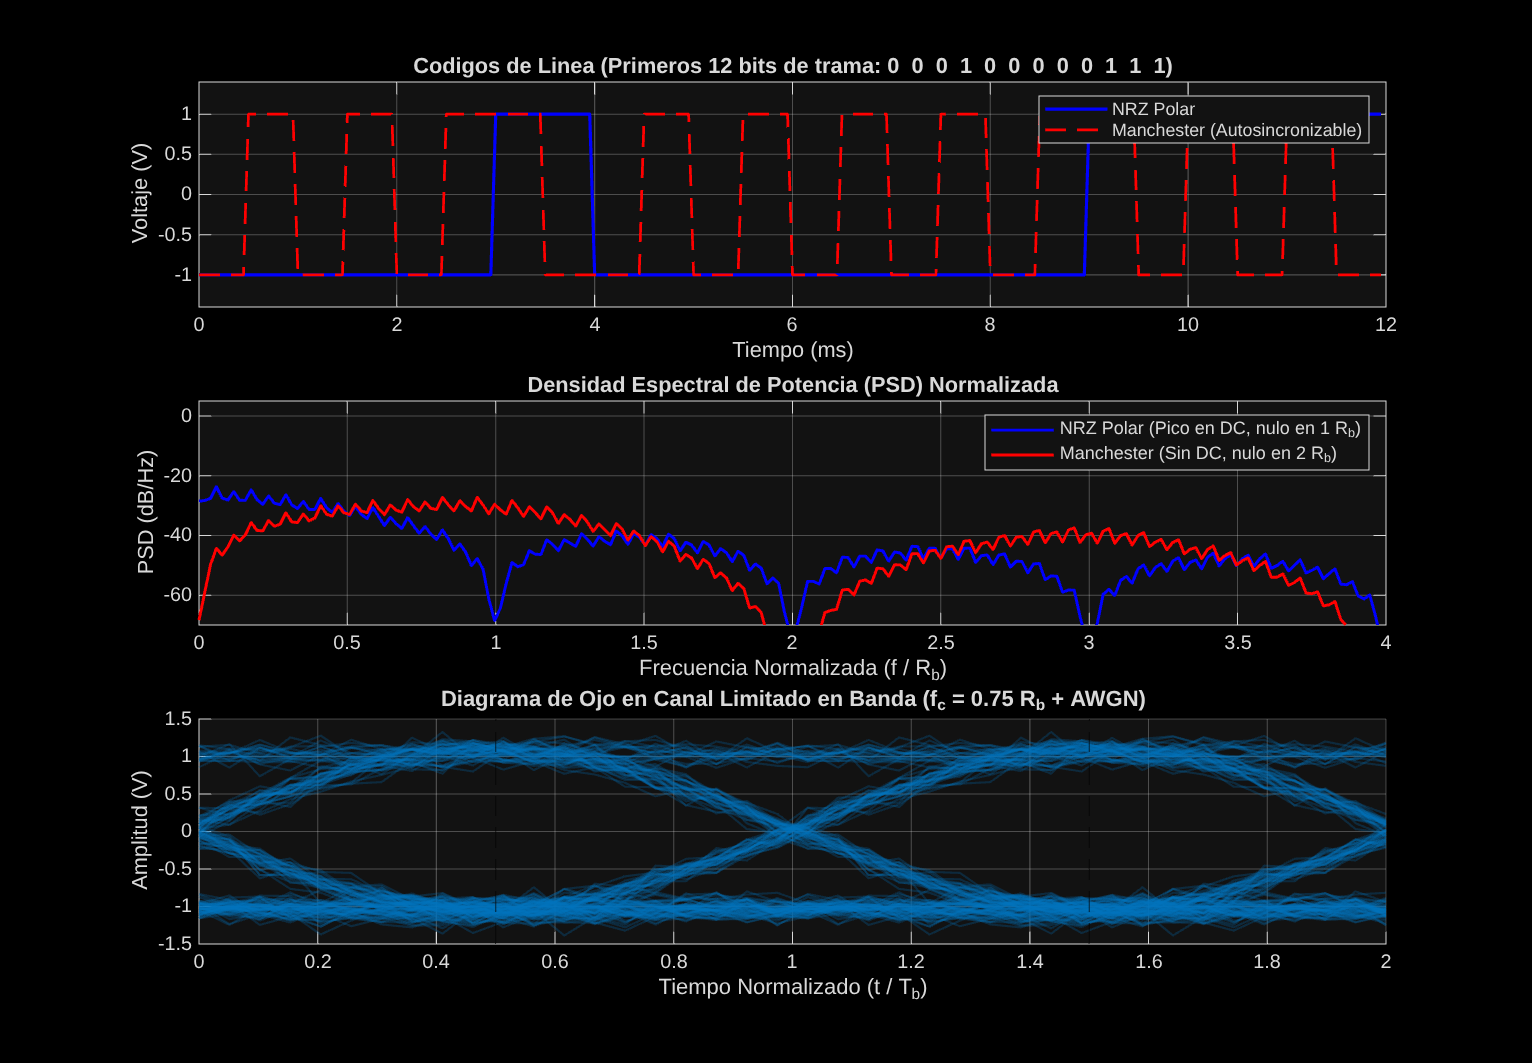
\includegraphics[width=0.92\textwidth]{figs/paso4_banda_base.png}
    \caption{Formas de onda NRZ Polar y Manchester, Densidad Espectral de Potencia (PSD) y diagrama de ojo con interferencia intersímbolo (ISI).}
    \label{fig:bandabase}
\end{figure}

\section{Entropía de Shannon y Compresión Huffman (Capítulo IV)}
Evaluando $N = 2000$ tramas de operación clínica, la fuente discreta de estados presenta una distribución no uniforme dominada por el estado \texttt{NORMAL} ($p_1 \approx 0.788$). La entropía de Shannon de la fuente está dada por:
\begin{equation}
H(X) = -\sum_{i=1}^{4} p(x_i)\log_2 p(x_i) \approx 1.078\text{ bits/símbolo}
\end{equation}
Al asignar palabras código de longitud variable mediante el algoritmo de Huffman (\texttt{'1'} para \texttt{NORMAL}, \texttt{'00'} para \texttt{ALERTA\_BAJA}, \texttt{'011'} para \texttt{ALERTA\_ALTA} y \texttt{'010'} para \texttt{SIN\_DETECCION}), la longitud promedio desciende de $2.00\text{ bits/símbolo}$ a $\bar{L} \approx 1.34\text{ bits/símbolo}$, alcanzando una eficiencia $\eta = H(X)/\bar{L} > 80\%$ y un ahorro neto de ancho de banda superior al $32\%$ sin pérdida de información.

\begin{figure}[H]
    \centering
    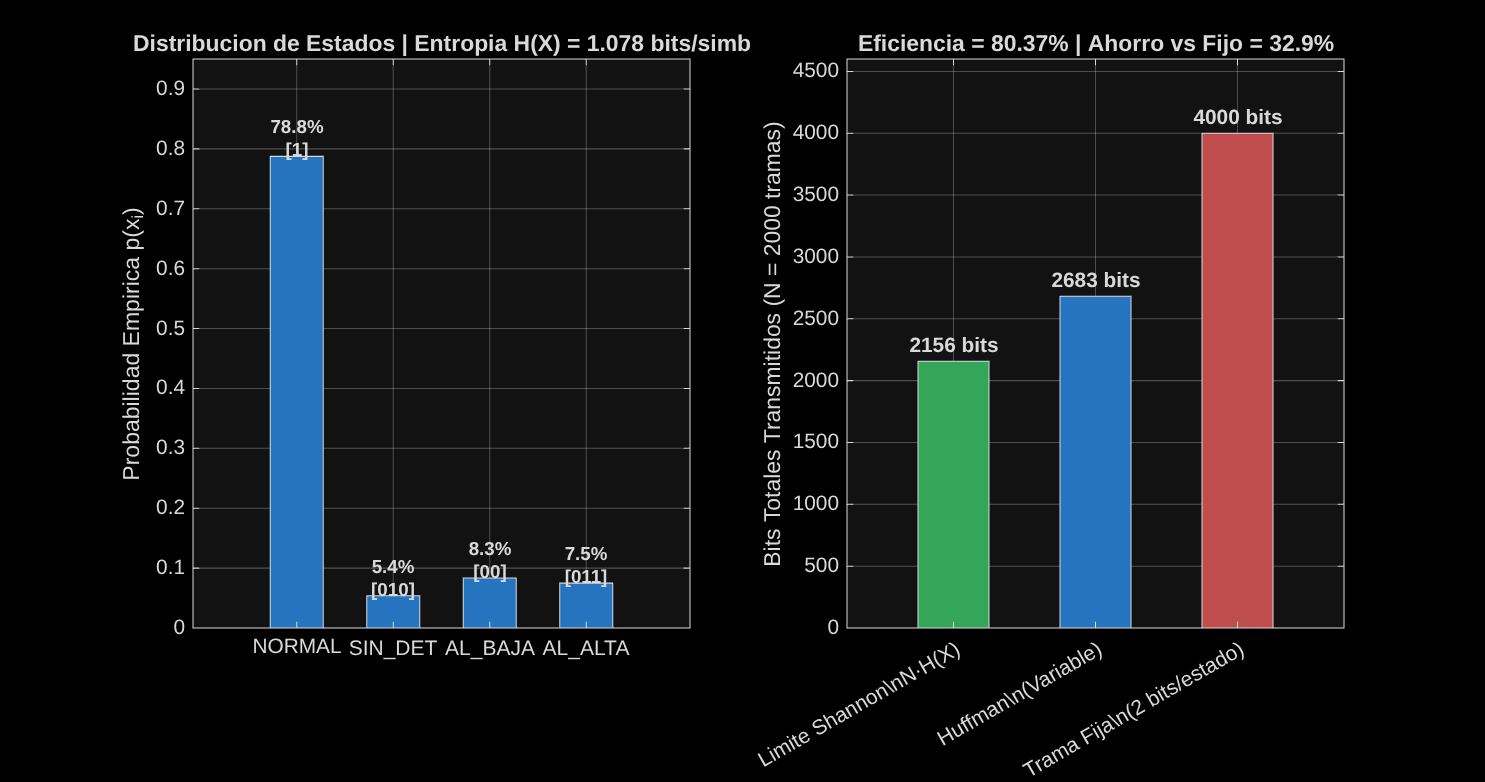
\includegraphics[width=0.92\textwidth]{figs/paso5_huffman.png}
    \caption{Distribución empírica de los estados del nodo sensor, códigos Huffman asignados y reducción total de bits transmitidos.}
    \label{fig:huffman}
\end{figure}

\section{Capacidad de Canal y Corrección de Errores Hamming (7,4) (Capítulo V)}
Para proteger las tramas binarias en enlaces inalámbricos ruidosos, se implementó un código lineal sistemático Hamming $(7,4)$ con tasa $R = k/n = 4/7$, matriz generadora $G = [I_4 \mid P]$ y matriz de verificación de paridad $H = [P^T \mid I_3]$. En el receptor, el vector de síndrome $\mathbf{s} = \mathbf{r}H^T \pmod{2}$ localiza y corrige automáticamente cualquier error simple por bloque de $7\text{ bits}$.

De acuerdo con el teorema de capacidad de canal de Shannon-Hartley, la eficiencia espectral máxima libre de error en un canal AWGN está acotada por:
\begin{equation}
\frac{C}{B} = \log_2(1 + \text{SNR})\text{ [bits/s/Hz]}
\end{equation}
Para $R = 4/7 \approx 0.571\text{ bits/s/Hz}$, el límite teórico mínimo es $\text{SNR}_{\min} = 2^{4/7} - 1 \approx -3.13\text{ dB}$. En simulación Monte Carlo con modulación BPSK antipodal, Hamming $(7,4)$ supera el umbral de cruce alrededor de $E_b/N_0 \approx 6.5\text{ dB}$ y reduce la tasa de error de bit (BER) a $0$ errores registrados en $E_b/N_0 = 10\text{ dB}$.

\begin{figure}[H]
    \centering
    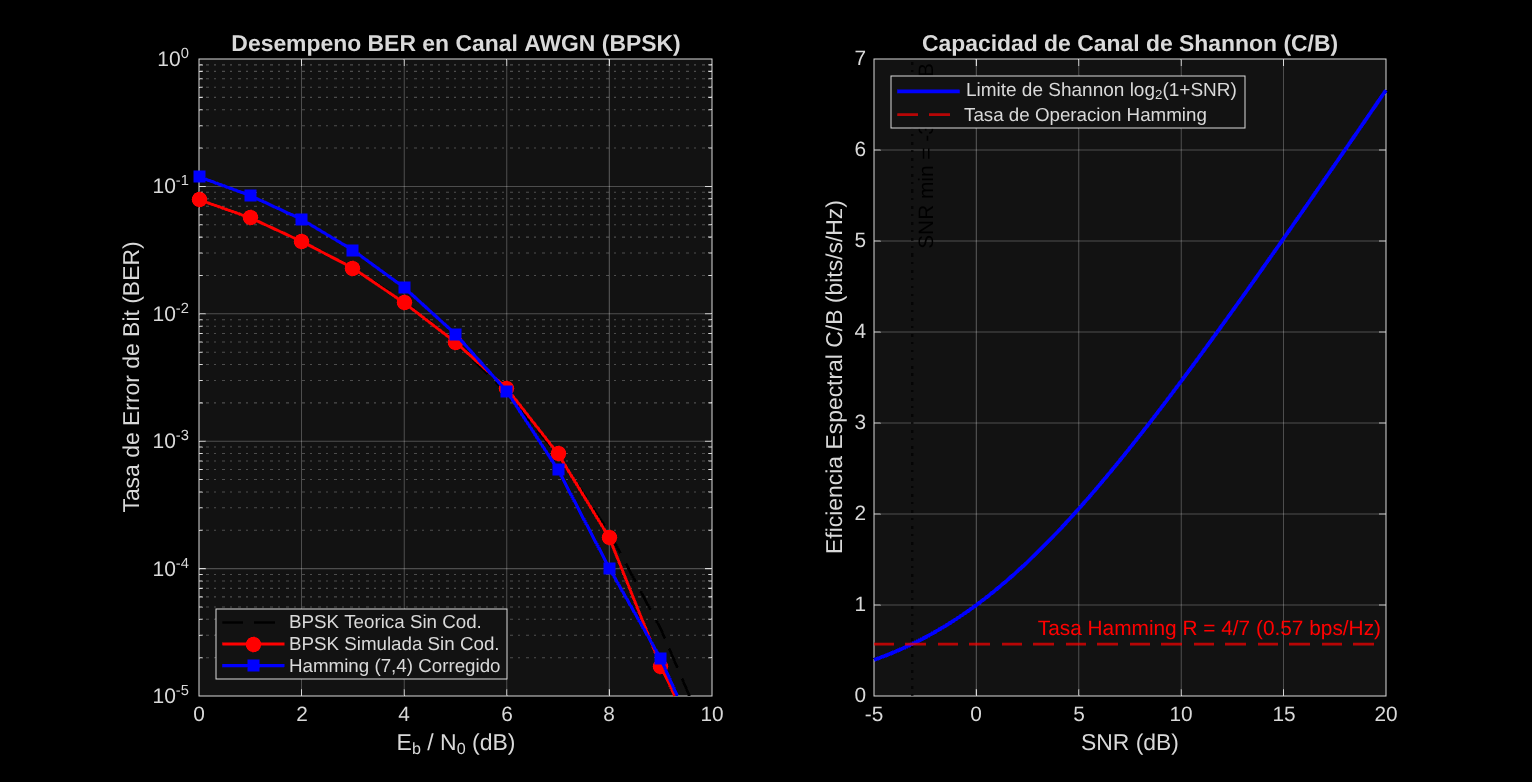
\includegraphics[width=0.92\textwidth]{figs/paso6_canal_hamming.png}
    \caption{Curvas de Tasa de Error de Bit (BER vs. $E_b/N_0$) en canal AWGN y límite de capacidad de Shannon $C/B$.}
    \label{fig:hamming}
\end{figure}

\section{Conclusiones}
La arquitectura modular implementada demuestra cómo el procesamiento digital de señales y la teoría de la información optimizan un sistema biomédico real: el filtrado pasa-banda acota el muestreo necesario a $F_s \ge 7.60\text{ Hz}$, la codificación de Huffman comprime en más de un $32\%$ las tramas de estado del paciente y el código Hamming $(7,4)$ garantiza integridad de datos en condiciones adversas de relación señal a ruido. Asimismo, el contrato de interfaz permite sustituir de forma inmediata los datos sintéticos por capturas seriales reales del ESP32-S3 Mini.

\end{document}
